%!TEX encoding=UTF-8
\documentclass[ 4paper,11pt,openany]{book}
\usepackage[T1]{fontenc}
\usepackage[english,italian]{babel}
\usepackage{graphicx}
\usepackage[margin=1in]{geometry}


\title{Progetto Lavoratori Stagionali}

\author{Christian Farina \\  Stefano Zenaro}
\date{anno 2021/2022}

\begin{document}
\frontmatter
\maketitle
\tableofcontents 

\mainmatter
\chapter{Introduzione}
Riassunto del progetto
 
\chapter{Struttura del progetto}%in questa parte metteremo i vari schemi
\section{Casi d'uso principali}
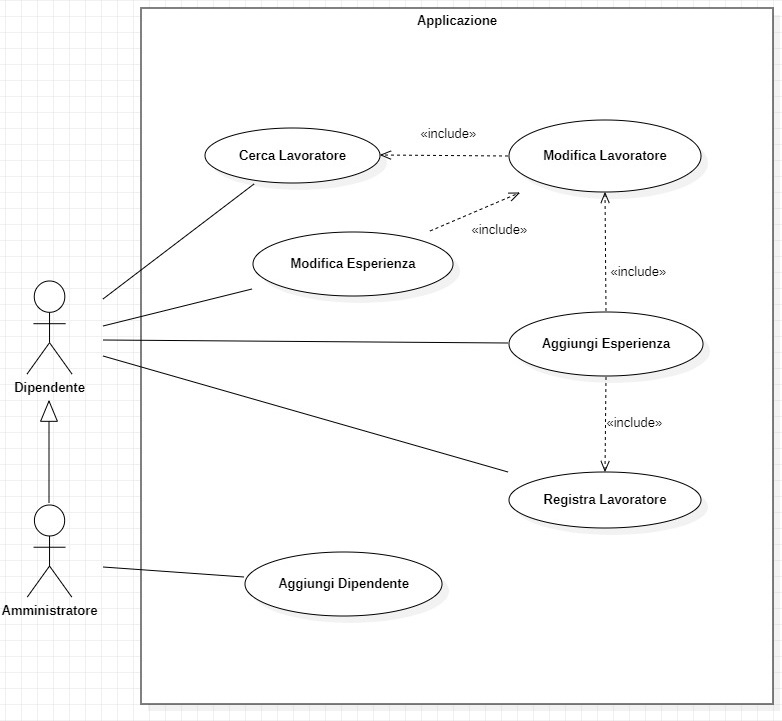
\includegraphics[width=180mm]{casi.jpg}
\section{Diagrammi di sequenza}
\subsection{Creazione e modifica di un lavoratore}
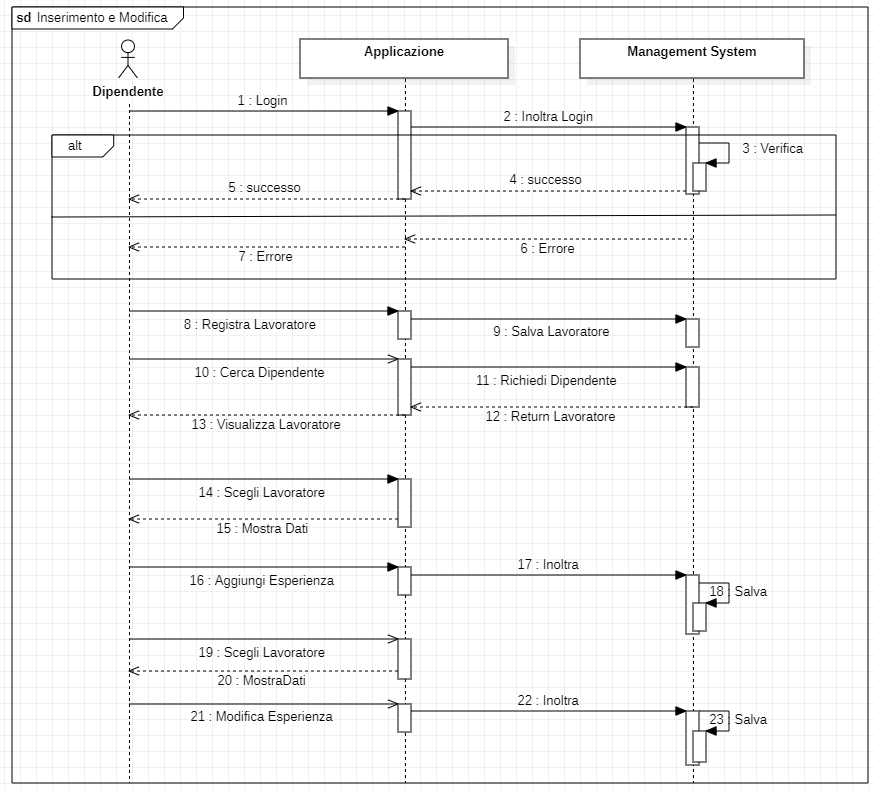
\includegraphics[width=180mm]{seq.png}
\subsection{Creazione di un dipendente}
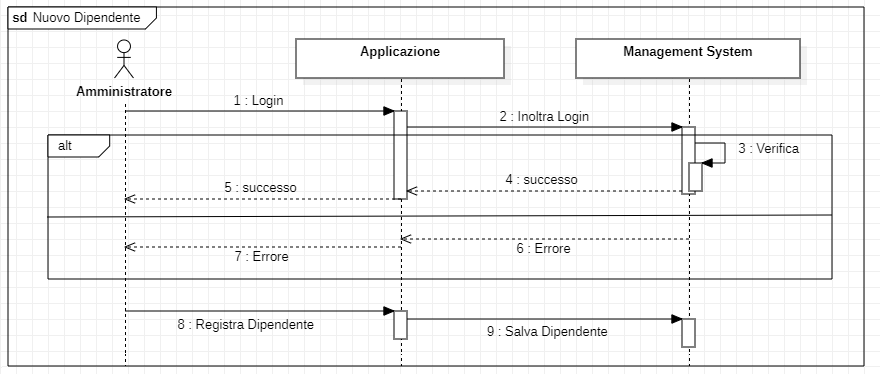
\includegraphics[width=180mm]{seq2.png}


\chapter{Implementazione}%in questa parte spiegheremo le robe di programmazione (pattern robe di progetto e minchiate varie)

\section{Pattern architetturale: MVC}
Per scrivere l'applicazione si e' deciso di implementare il pattern architetturale Model~View~Controller (MVC).

E' stato utilizzato il pattern MVC perche' permettere di separare le responsabilita' dell'applicazione in tre parti:
\begin{itemize}
    \item Model: il modello e' la logica interna della applicazione. Questa parte gestisce il login, l'inserimento, la ricerca e l'eliminazione dei dati, la lettura e la scrittura dei dati in modo permanente su disco.
    \item View: la vista e' la parte grafica che gestisce cio' che e' visibile dall'utente. Attraverso FXML e' possibile rappresentare pulsanti, tabelle e label.
    \item Controller: il controllore gestisce l'interazione dell'utente con l'interfaccia grafica permettendo la comunicazione tra la vista e il modello.
\end{itemize}

\section{Pattern di design: Singleton}
Per gestire creazione, elaborazione ed eliminazione dei dati e' stata creata una classe chiamata ManagementSystem che e' implementata seguendo il pattern Singleton.
Il pattern Singleton garantisce che all'interno della applicazione venga creata una sola istanza di questa classe.

Quando la classe viene istanziata viene eseguita la lettura dei file JSON e ad ogni inserimento o modifica dei dati questi vengono scritti su file.
Il vantaggio del pattern singleton applicato a questo approccio e' che permette di poter richiedere facilmente l'istanza all'interno di un qualsiasi controller garantendo che non sara' mai possibile avere stati indeterminati o multipli del sistema: e' sempre presente un unico stato che evolve nel tempo con la sua copia memorizzata su disco in formato JSON.

\chapter{Test}
Per testare il sistema sono stati implementati degli unit test per verificare il buon funzionamento di ogni metodo implementato nel modello.

\end {document}
